\documentclass[hints,nooutcomes,noauthor,handout]{ximera}

\graphicspath{  
{./}
{./whoAreYou/}
{./drawingWithTheTurtle/}
{./bisectionMethod/}
{./circles/}
{./anglesAndRightTriangles/}
{./lawOfSines/}
{./lawOfCosines/}
{./plotter/}
{./staircases/}
{./pitch/}
{./qualityControl/}
{./symmetry/}
{./nGonBlock/}
}


%% page layout
\usepackage[cm,headings]{fullpage}
\raggedright
\setlength\headheight{13.6pt}


%% fonts
\usepackage{euler}

\usepackage{FiraMono}
\renewcommand\familydefault{\ttdefault} 
\usepackage[defaultmathsizes]{mathastext}
\usepackage[htt]{hyphenat}

\usepackage[T1]{fontenc}
\usepackage[scaled=1]{FiraSans}

%\usepackage{wedn}
\usepackage{pbsi} %% Answer font


\usepackage{cancel} %% strike through in pitch/pitch.tex


%% \usepackage{ulem} %% 
%% \renewcommand{\ULthickness}{2pt}% changes underline thickness

\tikzset{>=stealth}

\usepackage{adjustbox}

\setcounter{titlenumber}{-1}

%% journal style
\makeatletter
\newcommand\journalstyle{%
  \def\activitystyle{activity-chapter}
  \def\maketitle{%
    \addtocounter{titlenumber}{1}%
                {\flushleft\small\sffamily\bfseries\@pretitle\par\vspace{-1.5em}}%
                {\flushleft\LARGE\sffamily\bfseries\thetitlenumber\hspace{1em}\@title \par }%
                {\vskip .6em\noindent\textit\theabstract\setcounter{question}{0}\setcounter{sectiontitlenumber}{0}}%
                    \par\vspace{2em}
                    \phantomsection\addcontentsline{toc}{section}{\thetitlenumber\hspace{1em}\textbf{\@title}}%
                     }}
\makeatother



%% thm like environments
\let\question\relax
\let\endquestion\relax

\newtheoremstyle{QuestionStyle}{\topsep}{\topsep}%%% space between body and thm
		{}                      %%% Thm body font
		{}                              %%% Indent amount (empty = no indent)
		{\bfseries}            %%% Thm head font
		{)}                              %%% Punctuation after thm head
		{ }                           %%% Space after thm head
		{\thmnumber{#2}\thmnote{ \bfseries(#3)}}%%% Thm head spec
\theoremstyle{QuestionStyle}
\newtheorem{question}{}



\let\freeResponse\relax
\let\endfreeResponse\relax

%% \newtheoremstyle{ResponseStyle}{\topsep}{\topsep}%%% space between body and thm
%% 		{\wedn\bfseries}                      %%% Thm body font
%% 		{}                              %%% Indent amount (empty = no indent)
%% 		{\wedn\bfseries}            %%% Thm head font
%% 		{}                              %%% Punctuation after thm head
%% 		{3ex}                           %%% Space after thm head
%% 		{\underline{\underline{\thmname{#1}}}}%%% Thm head spec
%% \theoremstyle{ResponseStyle}

\usepackage[tikz]{mdframed}
\mdfdefinestyle{ResponseStyle}{leftmargin=1cm,linecolor=black,roundcorner=5pt,
, font=\bsifamily,}%font=\wedn\bfseries\upshape,}


\ifhandout
\NewEnviron{freeResponse}{}
\else
%\newtheorem{freeResponse}{Response:}
\newenvironment{freeResponse}{\begin{mdframed}[style=ResponseStyle]}{\end{mdframed}}
\fi



%% attempting to automate outcomes.

%% \newwrite\outcomefile
%%   \immediate\openout\outcomefile=\jobname.oc
%% \renewcommand{\outcome}[1]{\edef\theoutcomes{\theoutcomes #1~}%
%% \immediate\write\outcomefile{\unexpanded{\outcome}{#1}}}

%% \newcommand{\outcomelist}{\begin{itemize}\theoutcomes\end{itemize}}

%% \NewEnviron{listOutcomes}{\small\sffamily
%% After answering the following questions, students should be able to:
%% \begin{itemize}
%% \BODY
%% \end{itemize}
%% }
\usepackage[tikz]{mdframed}
\mdfdefinestyle{OutcomeStyle}{leftmargin=2cm,rightmargin=2cm,linecolor=black,roundcorner=5pt,
, font=\small\sffamily,}%font=\wedn\bfseries\upshape,}
\newenvironment{listOutcomes}{\begin{mdframed}[style=OutcomeStyle]After answering the following questions, students should be able to:\begin{itemize}}{\end{itemize}\end{mdframed}}



%% my commands

\newcommand{\snap}{{\bfseries\itshape\textsf{Snap!}}}
\newcommand{\flavor}{\link[\snap]{https://snap.berkeley.edu/}}
\newcommand{\mooculus}{\textsf{\textbf{MOOC}\textnormal{\textsf{ULUS}}}}


\usepackage{tkz-euclide}
\tikzstyle geometryDiagrams=[rounded corners=.5pt,ultra thick,color=black]
\colorlet{penColor}{black} % Color of a curve in a plot



\ifhandout\newcommand{\mynewpage}{\newpage}\else\newcommand{\mynewpage}{}\fi

\title{Not so quick questions}


\author{Bart Snapp}

\begin{document}
\begin{abstract}
  We solve more difficult problems and revisit old ideas.
\end{abstract}
\maketitle


\begin{listOutcomes}
\item Apply the Pythagorean theorem to solve problems.
\item Extend ideas from two-dimensions to three-dimensions.
\item Follow steps in an algorithm to solve a problem.
\item Translate classroom mathematics into real world mathematics.
\item Recognize the difference between reasoning through formulas and
  reasoning through scaling.
\end{listOutcomes}


Imagine a house where the roof where two slopes meet. This will either
form a ``hip'' or a ``valley''.
\begin{center}
  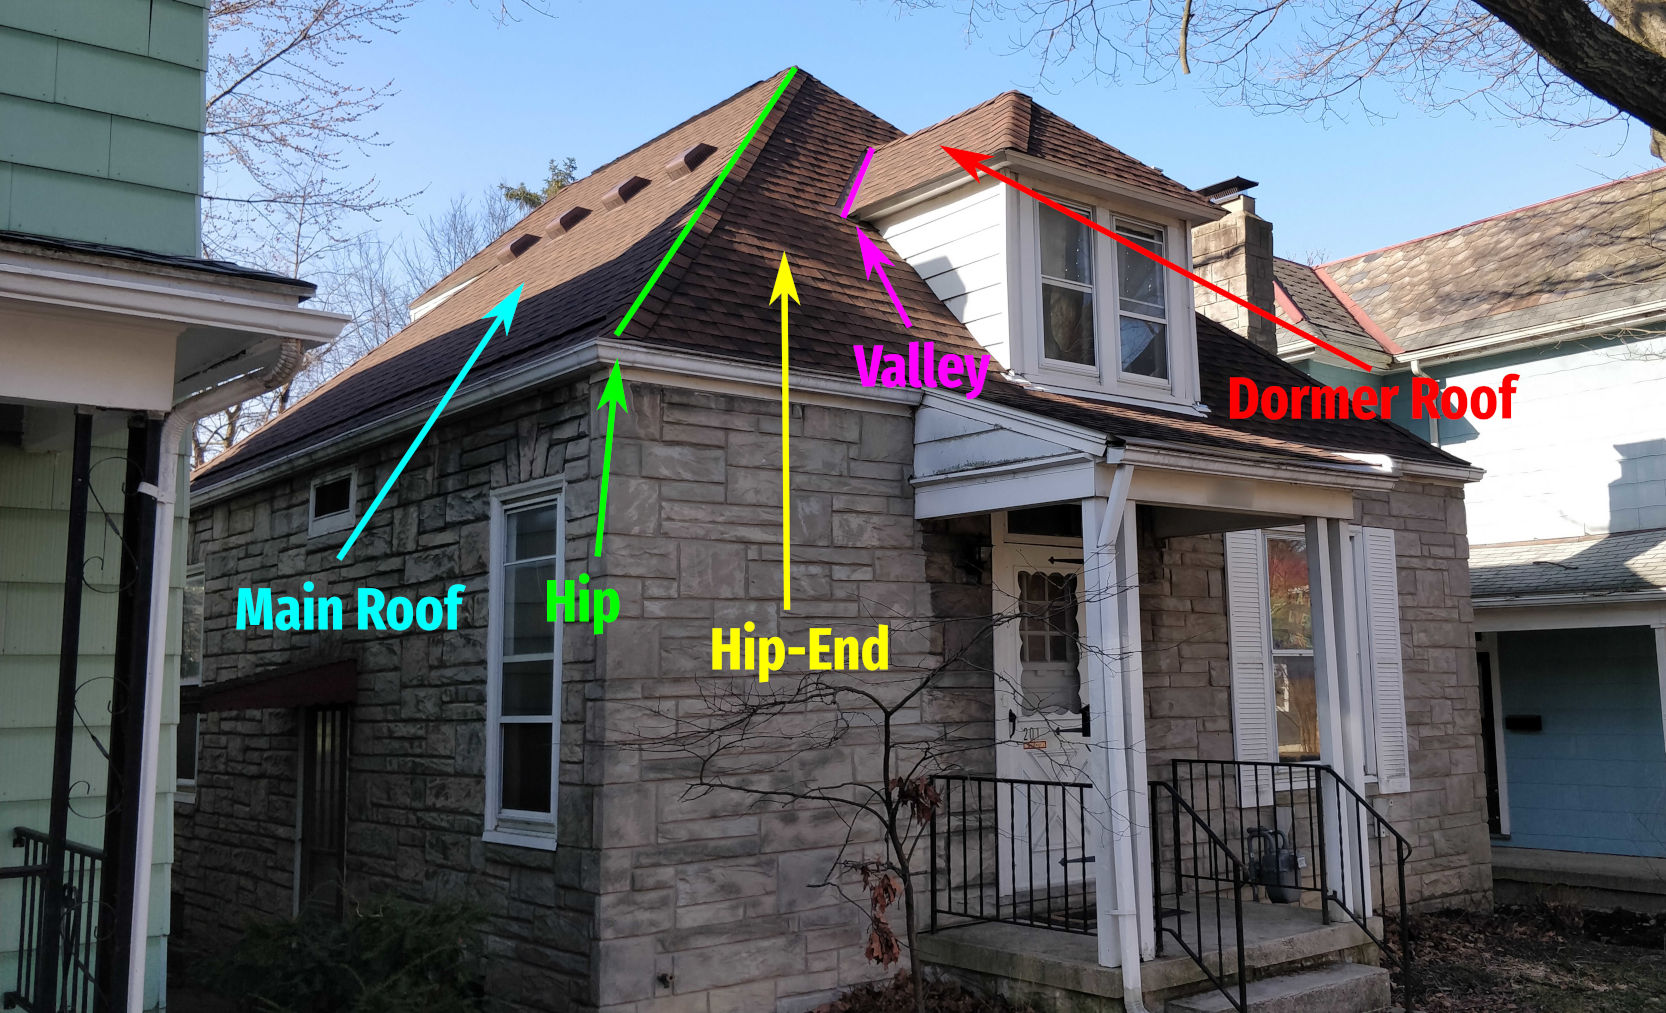
\includegraphics[width=.8\textwidth]{house.jpg}
\end{center}
There are two basic questions we'd like to answer about shapes like these:
\begin{itemize}
\item Given the dimensions (as seen from the top) of the roof, What is the AREA of the roof?
\item Given the SLOPE of the roofs that meet, What the slope (or
  pitch) of the hip or valley?
\end{itemize}


\mynewpage

\begin{question} We'll start by computing some areas.
\begin{enumerate}
\item Consider the \link[\textit{Luxor Las
    Vegas}]{https://en.wikipedia.org/wiki/Luxor_Las_Vegas}:
  \begin{center}
    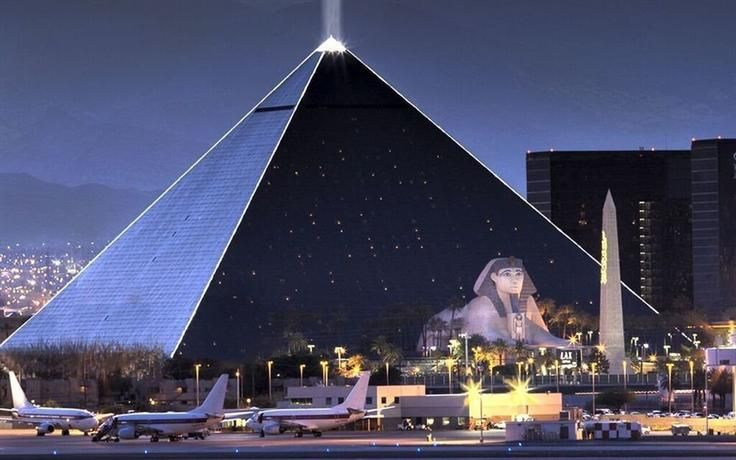
\includegraphics[width=.4\textwidth]{pyramid.jpg} 
  \end{center}
 Assuming that the (square) base of this building has a side length of
 $646$ feet and that the pyramid is $350$ feet tall, compute the
 SURFACE AREA in square feet, NOT including the bottom. 
 
\item Here are plans for a $1$-car garage that I got from \link[\textit{Garage Plans by Behm Design}]{https://behmdesign.com/shop/}:
   \begin{center}
     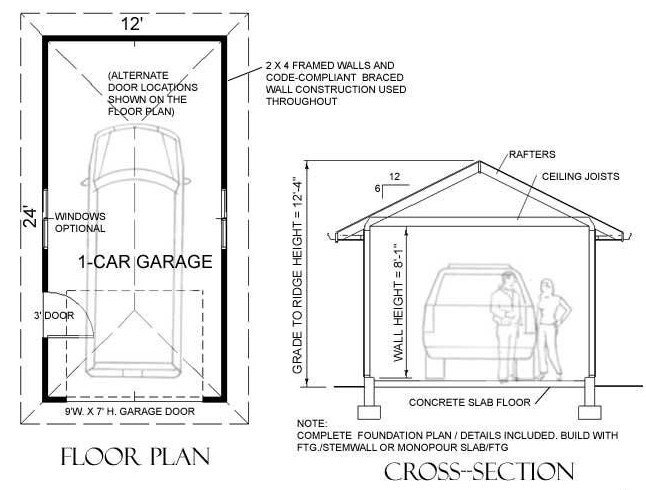
\includegraphics[width=.6\textwidth]{oneCarGarage.jpg}
   \end{center}
   Assuming that the hip-end has a slope of $\frac{6}{12}$, and that
   the roof has an overhang of $2$ feet on all sides, find the AREA of
   the roof of the garage in square feet.
 \item Considering the $1$-car garage from the previous part, now
   suppose that the hip-end has a slope of $\frac{8}{12}$ with an
   overhang of $2$ feet. Again find the AREA of the roof of the
   garage in square feet.
\end{enumerate}
In ALL cases above, SHOW and EXPLAIN your work.
\begin{freeResponse}
  \begin{enumerate}
    \item We must compute the height of one face of the pyramid. By
      the Pythagorean theorem, we have
      \[
      323^2 + 350^2 = h^2
      \]
      so
      \[
      h \approx 476.
      \]
      This means the top of the pyramid has a surface area of
      \[
      \text{Area} = 4\cdot \frac{646\cdot 476}{2} = 614992~\text{square feet}.
      \]
    \item Since there is an overhang of $2$ feet per side, the
      perimeter of the roof is a $16\times 28$ rectangle. If the main
      roof has a slope of $\frac{6}{12}$, it raises by
      \[
      8'\cdot \frac{6}{12}  = 4'
      \]
      This means that the height of both the main roof is $9'$ as
      measured along the roof. Moreover, we must move $8'$ in from the
      hip-end to achieve this height. Hence the main ridge is
      \[
      28-8-8 = 12~\text{feet}.
      \]
      Thus the area of the roof is
      \[
      2\cdot \underbrace{\frac{16\cdot 9}{2}}_{\text{hip-end}} +
      2\left(\underbrace{2\cdot \frac{8\cdot 9}{2} + 12\cdot
        9}_{\text{main roof}}\right) = 504 \text{square feet}.
      \]
    \item Since there is an overhang of $2$ feet per side, the
      perimeter of the roof is a $16\times 28$ rectangle. If the main
      roof has a slope of $\frac{6}{12}$, it raises by
      \[
      8'\cdot \frac{6}{12}  = 4'
      \]
      Again, the height of the main roof is
      \[
      \sqrt{8^2+4^2} = \sqrt{80}\approx 9'.
      \]
      Since the slope of the hip-end is $\frac{8}{12}$, and
      \begin{align*}
        x\cdot \frac{8}{12} &= 4\\
        x = \frac{12\cdot 4}{8}\\
        x = 6,
      \end{align*}
      thus must move $6'$ in from the hip-end to achieve this height.
      So the height of the hip-end (as measured along the roof) is
      \[
      \sqrt{6^2+4^2} = \sqrt{40} \approx 6.3'
      \]
      Finally, note that the length of the main ridge is
      \[
      28-6-6 = 16~\text{feet}.
      \]
      Thus the area of the roof is
      \[
      2\cdot \underbrace{\frac{16\cdot 6.3}{2}}_{\text{hip-end}} +
      2\left(\underbrace{2\cdot \frac{6\cdot 9}{2} + 16\cdot
        9}_{\text{main roof}}\right) = 496.8 \text{square feet}.
      \]
  \end{enumerate}
\end{freeResponse}


\end{question}
\mynewpage















\begin{question}
  Now let's think about the SLOPE of a hip or valley. Below we see a
  sneaky way to compute these numbers.
  \begin{mdframed}[style=OutcomeStyle]
\begin{quote}
  \textbf{Algorithm for computing the slope of a hip or valley:}

  Suppose the slopes are $\frac{s}{12}$ and $\frac{\l}{12}$ with
$s\le \l$.

\begin{enumerate}
\item Draw a point $O$ sitting at the intersection of a horizontal
  and vertical line.
\item Draw a vertical line segment $\bar{OS}$ where $S$ is directly
  above $O$ and $|OS| = s$.
  \item Starting from $S$, draw a line with the larger slope
    $\frac{\l}{12}$ and call the intersection of this line with the
    horizontal line point $X$.
  \item Starting at point $O$, extend the line segment $\bar{OS}$ by
    drawing downward $12$ units, and call the bottom of this segment
    $B$.
     \begin{center}
        \begin{tikzpicture}[geometryDiagrams,scale=.2]
          %% \filldraw[black] (1in,1in) circle (2pt) ;
          %% \filldraw[black] (0in,0in) circle (2pt) ;
          %% \filldraw[black] (0in,1in) circle (2pt) ;
          %% \draw[<->,dashed] (1.5in,-.5in) -- (-.5in,1.5in);

          \tkzDefPoint(0,0){O}
          \tkzDefPoint(-13,0){I}
          \tkzDefPoint(1,0){nI}
          \tkzDefPoint(0,7){II}
          \tkzDefPoint(0,-13){nII}
          
          \tkzDefPoint(0,6){S}
          \tkzDefPoint(-9,0){X}
          \tkzDefPoint(-12,-2){BS}
          \tkzDefPoint(0,-12){B}

          \tkzDrawPoint[](O)
          \tkzDrawPoint[](S)
          \tkzDrawPoint[](X)
          \tkzDrawPoint[](B)
          \tkzDrawLine[ultra thin](II,nII)
          \tkzDrawLine[ultra thin](I,nI)
          \tkzDrawLine(S,BS)
          \tkzDrawSegment(O,B)
          \tkzDrawSegment[ultra thick](B,X)
          \tkzDrawSegment(O,S)

          \tkzLabelPoint(O){$O$}
          \tkzLabelPoint[](S){$S$}
          \tkzLabelPoint[above left](X){$X$}
          \tkzLabelPoint(B){$B$}

          \draw[decoration={brace,raise=.2cm,mirror},decorate,thin] (S)--(X);
          
          \node[anchor=south east] at (-5,4) {slope of $\frac{\l}{12}$};
        \end{tikzpicture}
      \end{center}
  \item The slope you seek is:
    \[
    \frac{|OS|}{|BX|}\qquad \text{with a pitch of} \qquad \frac{12\cdot |OS|}{|BX|}
    \]  
\end{enumerate}
\end{quote}
  \end{mdframed}
  Let's see if we can USE the algorithm above.
  \begin{enumerate}
  \item Someone used this drawing to compute the slope of a hip.
    \begin{center}
        \begin{tikzpicture}[geometryDiagrams,scale=.2]
          %% \filldraw[black] (1in,1in) circle (2pt) ;
          %% \filldraw[black] (0in,0in) circle (2pt) ;
          %% \filldraw[black] (0in,1in) circle (2pt) ;
          %% \draw[<->,dashed] (1.5in,-.5in) -- (-.5in,1.5in);

          \tkzDefPoint(0,0){O}
          \tkzDefPoint(-13,0){I}
          \tkzDefPoint(1,0){nI}
          \tkzDefPoint(0,7){II}
          \tkzDefPoint(0,-13){nII}
          
          \tkzDefPoint(0,6){S}
          \tkzDefPoint(-9,0){X}
          \tkzDefPoint(-12,-2){BS}
          \tkzDefPoint(0,-12){B}

          \tkzDrawPoint[](O)
          \tkzDrawPoint[](S)
          \tkzDrawPoint[](X)
          \tkzDrawPoint[](B)
          \tkzDrawLine[ultra thin](II,nII)
          \tkzDrawLine[ultra thin](I,nI)
          \tkzDrawLine(S,BS)
          \tkzDrawSegment(O,B)
          \tkzDrawSegment[ultra thick](B,X)
          \tkzDrawSegment(O,S)


          \draw[decoration={brace,raise=.2cm,mirror},decorate,thin] (O)--(S);
          \node[anchor=west] at (1.5,3) {$6$};


          \draw[decoration={brace,raise=.2cm,mirror},decorate,thin] (B)--(O);
          \node[anchor=west] at (1.5,-6) {$12$};

          \draw[decoration={brace,raise=.2cm,mirror},decorate,thin] (S)--(X);
          \node[anchor=south east] at (-5,4) {slope of $\frac{8}{12}$};

          \draw[decoration={brace,raise=.2cm,mirror},decorate,thin] (X)--(B);
          \node[anchor=north east] at (-5,-6.5) {$15$};
        \end{tikzpicture}
    \end{center}
    Assuming that the slope of the main roof is LARGER than the slope
    of the hip-end, FIND the slopes (as a fraction over $12$) of the main-roof, the hip-end, and
    the hip. 
  \item Suppose you have a main-roof with a slope of $\frac{4}{12}$
    and a hip-end with a slope of $\frac{7}{12}$. Either draw a
    careful picture OR use
    \link[\textit{GeoGebra}]{https://www.geogebra.org/classic} to
    \textbf{find the slope of the hip.}  Show all work, explain your
    reasoning, and check your work with an \link[online
      calculator]{https://www2.strongtie.com/webapps/SlopeSkew/?source=app}.
  \item If the slope of the main roof is the same as the slope of the
    hip-end, say they are both $\frac{s}{12}$, what is the slope of
    the hip? Show all work and explain your reasoning.
  \end{enumerate}
  \begin{freeResponse}
    \begin{enumerate}
    \item The slope of the main roof is $\frac{6}{12}$. The slope of
      the hip-end is $\frac{8}{12}$. The slope of the hip is
      \[
      \frac{6}{15} \approx \frac{4.8}{12}.
      \]
    \item Using \textit{GeoGebra} we find:
      \begin{center}
        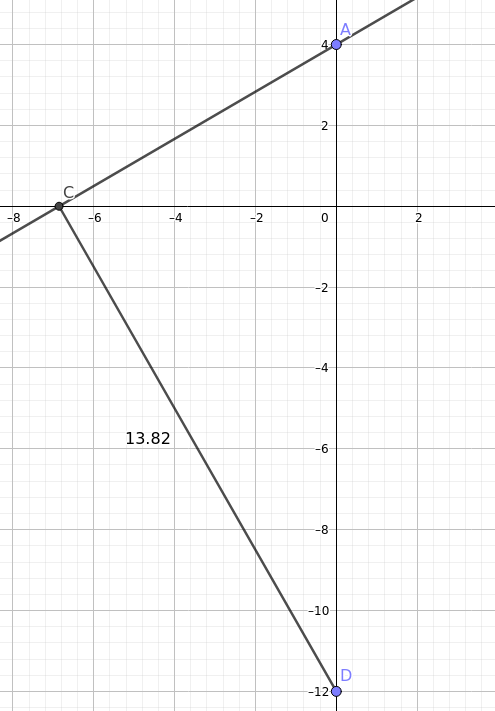
\includegraphics[width=.3\textwidth]{workUnEqSlope.png}
      \end{center}
      Hence the slope is
      \[
      \frac{4}{13.82} \approx \frac{3.5}{12}.
      \]
    \item If both slopes are the same, then our picture looks like
      this:
      \begin{center}
        \begin{tikzpicture}[geometryDiagrams,scale=.2]
          %% \filldraw[black] (1in,1in) circle (2pt) ;
          %% \filldraw[black] (0in,0in) circle (2pt) ;
          %% \filldraw[black] (0in,1in) circle (2pt) ;
          %% \draw[<->,dashed] (1.5in,-.5in) -- (-.5in,1.5in);

          \tkzDefPoint(0,0){O}
          \tkzDefPoint(-13,0){I}
          \tkzDefPoint(1,0){nI}
          \tkzDefPoint(0,7){II}
          \tkzDefPoint(0,-13){nII}
          
          \tkzDefPoint(0,6){S}
          \tkzDefPoint(-12,0){X}
          \tkzDefPoint(-12,0){BS}
          \tkzDefPoint(0,-12){B}

          \tkzDrawPoint[](O)
          \tkzDrawPoint[](S)
          \tkzDrawPoint[](X)
          \tkzDrawPoint[](B)
          \tkzDrawLine[ultra thin](II,nII)
          \tkzDrawLine[ultra thin](I,nI)
          \tkzDrawLine(S,BS)
          \tkzDrawSegment(O,B)
          \tkzDrawSegment[ultra thick](B,X)
          \tkzDrawSegment(O,S)

          \tkzLabelPoint(O){$O$}
          \tkzLabelPoint[](S){$S$}
          \tkzLabelPoint[above left](X){$X$}
          \tkzLabelPoint(B){$B$}

          \draw[decoration={brace,raise=.2cm,mirror},decorate,thin] (S)--(X);
          
          \node[anchor=south east] at (-5,4) {slope of $\frac{s}{12}$};

          \draw[decoration={brace,raise=.2cm,mirror},decorate,thin] (X)--(B);
          \node[anchor=north east] at (-6,-6.5) {$\sqrt{12^2+12^2}$};
        \end{tikzpicture}
      \end{center}
      So the slope we see seek is
      \[
      \frac{s}{\sqrt{12^2+12^2}} =  \frac{s}{12\sqrt{2}} = \frac{s/\sqrt{2}}{12}.
      \]
    \end{enumerate}
  \end{freeResponse}
\end{question}




\mynewpage


\begin{question}
  Now let's reflect on the content above a bit.
  \begin{enumerate}
    \item EXPLAIN using words, pictures, and so on, as needed/helpful,
      WHY computing the \textbf{slope of a hip} is the SAME as computing the
      \textbf{slope of a valley}.
    \item If all the slopes of a roof are the same, say $s/12$, there
      is an even easier method of finding the area of the roof using
      SCALING. Discover this method, and demonstrate that it is
      correct by using it to give a NEW SOLUTION to Problem $1$, part
      $(b)$ above.
  \end{enumerate}
  \begin{freeResponse}
    \begin{enumerate}
  \item A hip is just an ``upside-down'' valley, and the slopes are
    the same.
  \item If the slope is $\frac{s}{12}$, we multiply the area of the
    roof (as seen from above) by
    \[
    \frac{\sqrt{s^2+12^2}}{12}.
    \]
    check it out:
    \[
    16\cdot 28 = 448,\qquad\text{and}\qquad  16\cdot 28 \frac{\sqrt{s^2+12^2}}{12} \approx 500.
    \]
    This is different from our previous answers due to rounding.
    \end{enumerate}
  \end{freeResponse}
\end{question}

\end{document}
